%% Manuscript for the Journal of Functional Programming (Episciences), class jfp-epi v1.2.
%% Submission draft: the `review' option adds the mandatory line numbers and the
%% "DRAFT PAPER UNDER REVIEW" footer. For an arXiv/HAL/Zenodo copy, remove `review'
%% (the journal's instructions: arXiv does not allow line numbers).
\documentclass[review]{jfp-epi}

\usepackage{listings}
\usepackage{booktabs}
\usepackage{tikz}
\usetikzlibrary{arrows.meta,positioning,fit,backgrounds}

\lstset{
  language=Haskell,
  basicstyle=\ttfamily\footnotesize,
  columns=fullflexible,
  keepspaces=true,
  showstringspaces=false,
  frame=single,
  framerule=0.2pt,
  xleftmargin=0.5em,
  xrightmargin=0.5em,
  aboveskip=0.8em,
  belowskip=0.6em,
  breaklines=true,
  literate={->}{{$\to$}}1 {=>}{{$\Rightarrow$}}1
}

\newcommand{\crem}{\texttt{crem}}
\newcommand{\code}[1]{\texttt{#1}}

\begin{document}

\title{Limits of type-level transition guarantees in composable state machines: a closed-loop case study in Haskell}

%% TODO(author): ORCIDs are required for all authors on JFP submissions (class guide, Sec. 2);
%% add \orcid{...} after \author{...}. Decide whether the advisor is a co-author and add the e-mail.
\author{Peterson Carara Junior}
\affiliation{%
  \institution{Faculdade de Tecnologia da Baixada Santista ``Rubens Lara'' (Fatec BS)}
  \city{Santos}
  \state{SP}
  \country{Brazil}
  \authoremail{[e-mail to be added]}
}

\begin{abstract}
Typed state-machine libraries promise that illegal transitions do not compile. We ask what that guarantee is worth once machines are composed. Using the \crem{} library for Haskell, we study a four-state avionics machine composed with a battery machine and a reactive environment closed by \code{Feedback}. The domain is an illustrative discrete case study; we make no claim about real avionics. A rejection matrix over all 16 vertex pairs and nine mutants of the implementation show that the checker rejects edges outside the topology and omitted cases written without a wildcard, but accepts a wrong destination on an allowed edge, swapped events, wrong outputs, faulty environments and an omission hidden by a catch-all clause, which only tests catch. We then describe a validation method that other \crem{} users can reuse: a reviewable transition table with the provenance of each rule, a table-driven oracle, a typed boundary adapter, property-based testing with Hedgehog, and an exhaustive exploration of the closed-loop state graph that runs the real \crem{} machines from any triple of vertices. Under a stated abstraction hypothesis, the exploration establishes equivalence between implementation and oracle for sequences of any length, and exposes a global defect that every edge-level check misses: the environment reacts to the \emph{edge} ``the battery became critical'' and not to the \emph{level}, so the aircraft can stay airborne with a critical battery forever. A TLA+ model checked with TLC independently reproduces the finding. The defect belongs to the environment model, not to \crem{}; the lesson is where the type-level guarantee stops.
\end{abstract}

\maketitle

\section{Introduction}

Finite-state machines are a standard way to specify reactive behaviour, and a long line of work asks how to make a programming language enforce the specification. In a pure functional language the machine becomes a function from state and event to a new state, algebraic data types make the sets of states and events closed, and the compiler checks that the transition function covers every pair \cite{hutton2016haskell,malakhovski2009fsm}. Libraries such as \texttt{motor} \cite{motor} and \crem{} \cite{perone2023crem} go further: they lift the allowed transitions to the type level, so that an action that returns a destination not permitted from its origin fails to type-check.

This is a real guarantee, and it is local. It says that \emph{each edge} used by the code is in a declared topology. It does not say which event causes which edge, and it says nothing about what happens when several machines are composed and fed back to one another. Perone and Karachalias themselves list, among the limitations of \crem{}, that the topology is not tied to the inputs that trigger the transitions \cite{perone2023crem}. The practical question is therefore: \emph{what does an engineer still have to verify after the compiler is satisfied, and how can that be done in the same language?}

We answer it with a small, fully worked case study and a method.

\paragraph{Case study.} A four-state avionics machine (\code{Grounded}, \code{InFlight}, \code{EmergencyLanding}, \code{Shutdown}), a three-level battery machine, and a reactive environment that observes their outputs and feeds events back one tick later. The system is built with \crem{}'s \code{Parallel} and \code{Feedback}. It is an illustration chosen to exercise composition; there are no real flight-safety requirements behind it, and we make no claim about real avionics.

\paragraph{Contributions.}
\begin{enumerate}
\item A precise delimitation of what the \crem{} type checker enforces in this case study (Sect.~\ref{sec:guarantee}): a rejection matrix over all 16 pairs of vertices with the \emph{cause} of each rejection checked, and nine mutants of the implementation, two refused by the compiler and seven accepted and killed only by tests.
\item A reusable validation method (Sect.~\ref{sec:method}): a reviewable transition table that records, for each rule, whether it comes from the requirements, from a project convention or from a modelling choice; an oracle driven by that table; a typed adapter for external input; and property-based testing with reproducible seeds and shrinking.
\item An exhaustive exploration of the closed-loop state graph that executes the \emph{real} \crem{} machines from an arbitrary triple of vertices (Sect.~\ref{sec:reach}). Under a stated hypothesis, it replaces bounded enumeration by a statement about sequences of any length.
\item A finding that no edge-level check can make: a reachable blind state in which the aircraft stays airborne with a critical battery forever (Sect.~\ref{sec:results}), reproduced independently by a TLA+ model checked with TLC.
\end{enumerate}

\paragraph{What this paper does not claim.} It introduces no new type system, no formal semantics and no general proof that composition preserves the guarantees of its parts. The environment is a modelling choice of the author, and the defect we report is a property of that model, not of \crem{} or of GHC. The table, the oracle and the TLA+ specification were written by the same person who wrote the implementation: the independence we obtain is of \emph{code}, not of \emph{authorship} (Sect.~\ref{sec:threats}).

Section~\ref{sec:background} reviews \crem{}, Sect.~\ref{sec:case} introduces the case study, Sect.~\ref{sec:guarantee} delimits the guarantee, Sect.~\ref{sec:method} presents the method, Sect.~\ref{sec:results} the results, Sect.~\ref{sec:discussion} the lessons and threats, and Sect.~\ref{sec:related} related work.

\section{Background: topologies and composition in crem}
\label{sec:background}

A \crem{} machine is a Mealy machine: on each input it emits an output and updates its state. The vertices of the state graph are promoted to the type level with the \code{singletons} library \cite{eisenberg2012singletons}, and the \emph{topology} is a value listing, for each vertex, the vertices that may follow it. Listing~\ref{lst:topology} shows the avionics machine. The action receives the current vertex as a singleton and returns an \code{ActionResult} built by \code{pureResult}, which demands the constraint \code{AllowedTransition topology from to}.

\begin{lstlisting}[float=t,caption={Topology and action of the avionics machine (excerpt).},label={lst:topology}]
$(singletons [d|
  data AvionicsVertex = Grounded | InFlight | EmergencyLanding | Shutdown
  avionicsTopology :: Topology AvionicsVertex
  avionicsTopology = Topology
    [ (Grounded,         [InFlight, Shutdown])
    , (InFlight,         [EmergencyLanding])
    , (EmergencyLanding, [Grounded]) ] |])

avionicsAction :: Applicative m => SAvionicsVertex v -> AvEvent
               -> ActionResult m AvionicsTopology SAvionicsVertex v Output
avionicsAction SGrounded TakeoffSignal   = pureResult MsgTakeoff   SInFlight
avionicsAction SInFlight CriticalBattery = pureResult MsgEmergency SEmergencyLanding
-- ... 16 equations in total, none with a wildcard
\end{lstlisting}

\paragraph{How the constraint is solved.} In \code{crem} 0.1.0.0, \code{AllowedTransition} has four instances, all marked \code{INCOHERENT}: one succeeds when the edge is the first in the origin's list, one skips the first edge of the origin, one skips the first vertex of the topology, and one for the identity edge. Resolution is thus a search for any path that closes the proof, and a missing edge leaves a residual constraint over the empty list. The identity edge is always allowed, so an event that must not change the state is written by returning the same vertex. We did not prove that this resolution is correct for every topology; for ours it agrees with the specification on all 16 pairs (Sect.~\ref{sec:guarantee}).

\paragraph{Composition.} Machines are the leaves (\code{Basic}) of a tree whose nodes are \code{Sequential}, \code{Parallel}, \code{Alternative}, \code{Feedback} and \code{Kleisli}. Each leaf keeps its own state and topology. \code{Feedback} runs the forward machine on an input, passes each output to the return machine, and re-injects every input that the return machine emits, recursively, until it emits nothing. This makes \code{Feedback} \emph{instantaneous} within one call of \code{run}; any delay has to be modelled, as we do below.

\section{The case study}
\label{sec:case}

\paragraph{The avionics machine.} Table~\ref{tab:delta} gives its transition function. Only four rows come from the requirement text (marked \texttt{R}); the other twelve pairs are a project convention (the state does not change and the output is \code{MsgIgnored}), because the text does not say what happens there. The output names are also a convention. The one prohibition in the requirements is the direct edge from \code{InFlight} to \code{Shutdown}.

\begin{table}[t]
\caption{Transition function of the avionics machine. \texttt{R}: stated in the requirement text; unmarked cells keep the state (project convention) and output \code{MsgIgnored}.}
\label{tab:delta}
\footnotesize
\setlength{\tabcolsep}{3pt}
\begin{tabular}{@{}lllll@{}}
\toprule
State & \code{TakeoffSignal} & \code{CriticalBattery} & \code{LandedSignal} & \code{SystemCutoff} \\
\midrule
\code{Grounded}         & \code{InFlight} (R) & -- & -- & \code{Shutdown} (R) \\
\code{InFlight}         & -- & \code{EmergencyLanding} (R) & -- & -- \\
\code{EmergencyLanding} & -- & -- & \code{Grounded} (R) & -- \\
\code{Shutdown}         & -- & -- & -- & -- \\
\bottomrule
\end{tabular}
\end{table}

\paragraph{The battery machine.} Three levels (\code{Charged}, \code{Low}, \code{Critical}); \code{Drain} goes one level down, \code{Recharge} one up, and \code{ShedLoad} (a load shedding that only relieves \code{Critical} to \code{Low}) was added for the closed loop. There is no edge from \code{Charged} to \code{Critical}. Every rule of this machine is a modelling choice.

\paragraph{The environment and the loop.} The plant is the \code{Parallel} composition of the two machines. A third machine, \code{Mission}, observes their telemetry and closes the loop with \code{Feedback} (Fig.~\ref{fig:loop}). Because \code{Feedback} is instantaneous, the one-tick delay is obtained by making \code{Mission} a \emph{one-slot register}: relevant telemetry makes it \emph{hold} an event, and the \code{Beat} that opens the next tick makes it \emph{release} the held event. Concretely, a critical battery is held as \code{CriticalHeld} and released as \code{CriticalBattery} to the avionics; \code{MsgEmergency} is held as \code{TouchdownHeld} and released as \code{ShedLoad} to the battery followed by \code{LandedSignal}; \code{MsgLanded} is held as \code{CutoffHeld} and released as \code{SystemCutoff}. While the slot is occupied, new telemetry is \emph{dropped}. A tick processes the \code{Beat}, then the command, then the battery event, and every signal released during a tick is processed, depth first, before the next external signal.

\begin{figure}[t]
\centering
\footnotesize
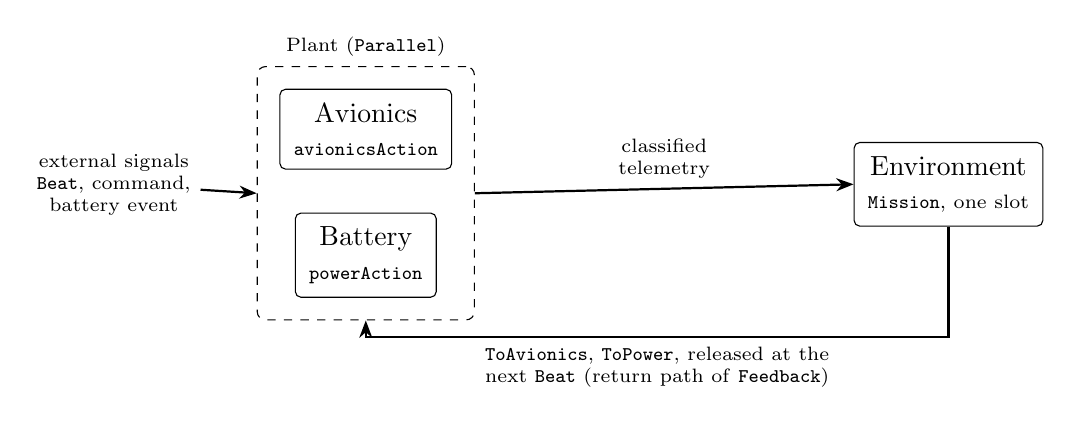
\begin{tikzpicture}[
    box/.style={draw, rounded corners=2pt, minimum height=0.9cm, align=center, inner sep=5pt},
    ar/.style={-{Stealth[length=2.2mm]}, thick},
    lb/.style={font=\scriptsize, align=center}
]
\node[box] (av) at (0,0.7) {Avionics\\{\scriptsize\code{avionicsAction}}};
\node[box] (pw) at (0,-0.9) {Battery\\{\scriptsize\code{powerAction}}};
\begin{scope}[on background layer]
\node[draw, dashed, rounded corners=3pt, fit=(av)(pw), inner sep=8pt, label={[font=\scriptsize]above:Plant (\code{Parallel})}] (plant) {};
\end{scope}
\node[box] (mis) at (7.4,0) {Environment\\{\scriptsize\code{Mission}, one slot}};
\node[lb] (ext) at (-3.2,0) {external signals\\{\scriptsize\code{Beat}, command,}\\{\scriptsize battery event}};
\draw[ar] (ext) -- (plant.west);
\draw[ar] (plant.east) -- node[lb, above] {classified\\telemetry} (mis.west);
\draw[ar] (mis.south) -- ++(0,-1.4) -| node[lb, pos=0.25, below] {\code{ToAvionics}, \code{ToPower}, released at the\\next \code{Beat} (return path of \code{Feedback})} (plant.south);
\end{tikzpicture}
\caption{The closed loop. The environment holds relevant telemetry and releases it at the next tick.}
\label{fig:loop}
\end{figure}

Listing~\ref{lst:mission} shows three of the 20 equations of \code{Mission}; the last one is the one that matters later.

\begin{lstlisting}[caption={Excerpt of the environment machine.},label={lst:mission}]
missionAction SStandby CueBatteryCritical
  = pureResult [] SCriticalHeld
missionAction SCriticalHeld CueBeat
  = pureResult [ToAvionics CriticalBattery] SStandby
missionAction SCriticalHeld CueBatteryCritical
  = pureResult [] SCriticalHeld   -- slot busy: dropped
\end{lstlisting}

\paragraph{Three environment policies.} \code{OneSlot} is the implementation above. \code{Queue} is a loss-free variant in which each kind of held event enters once. \code{Level} is \code{OneSlot} plus a reaction to the battery \emph{level}: on each \code{Beat}, with the slot free, the battery in \code{Critical} and the avionics \code{InFlight}, it releases \code{CriticalBattery}. Only \code{OneSlot} exists in \crem{}; the other two exist in the oracle.

\section{What the type checker does and does not guarantee}
\label{sec:guarantee}

\subsection{Rejection matrix}

For each of the 16 ordered pairs of vertices we generate a minimal module whose action returns the destination from the origin, and compile it. The expected outcome is derived from the transition table, not from a hand-written list: the four edges and the four identities compile, the other eight pairs must be rejected. A pair counts as rejected only if GHC reports exactly one error and that error is \code{Could not deduce AllowedTransition} naming the pair; any other failure is a mismatch. All 16 results agree with the table (Table~\ref{tab:matrix}).

\begin{table}[t]
\caption{Compilation of \code{pureResult} for every (origin, destination) pair. \checkmark: compiles (identity on the diagonal); $\times$: rejected with the expected cause.}
\label{tab:matrix}
\small
\begin{tabular}{@{}lcccc@{}}
\toprule
origin $\backslash$ destination & \code{Grounded} & \code{InFlight} & \code{EmergencyLanding} & \code{Shutdown} \\
\midrule
\code{Grounded}         & \checkmark & \checkmark & $\times$ & \checkmark \\
\code{InFlight}         & $\times$ & \checkmark & \checkmark & $\times$ \\
\code{EmergencyLanding} & \checkmark & $\times$ & \checkmark & $\times$ \\
\code{Shutdown}         & $\times$ & $\times$ & $\times$ & \checkmark \\
\bottomrule
\end{tabular}
\end{table}

This matrix checks the \emph{topology}. It is not the same as the origin-by-event matrix, which also has 16 cells but checks that the transition function covers every pair. That second property is, in GHC, a warning (\code{-Wincomplete-patterns}) and only becomes a compile error if the project asks for it; we compile with \code{-Werror=incomplete-patterns} and write all 16 equations without a wildcard, since a wildcard would hide an omission (mutant H9 below).

\subsection{Mutation of the implementation}

To learn which defects the checker \emph{cannot} see, we injected nine defects, one at a time, into a temporary copy of the code and ran every test suite on each (Table~\ref{tab:mutants}).

\begin{table}[t]
\caption{Mutants of the \crem{} implementation. ``Accepted'' means that the compiler accepts the mutant.}
\label{tab:mutants}
\footnotesize
\begin{tabular}{@{}lp{5.2cm}lp{2.2cm}@{}}
\toprule
Id & Defect & Compiler & Killed by \\
\midrule
H1 & illegal edge \code{InFlight}$\to$\code{Shutdown} in topology and action & accepted & all five suites \\
H2 & wrong destination on an allowed edge (\code{Grounded}, \code{TakeoffSignal} $\to$ \code{Shutdown}) & accepted & all five \\
H3 & swapped events in \code{Grounded} (\code{TakeoffSignal}, \code{SystemCutoff}) & accepted & all five \\
H4 & illegal action \emph{without} changing the topology & \textbf{rejected} & -- \\
H5 & omitted (state, event) pair & \textbf{rejected} (exhaustiveness as error) & -- \\
H6 & wrong output (\code{EmergencyLanding}, \code{LandedSignal} emits \code{MsgIgnored}) & accepted & four suites \\
H7 & environment: \code{CriticalHeld} releases \code{LandedSignal} & accepted & three suites \\
H8 & battery: \code{Low} with \code{Drain} stays \code{Low} & accepted & four suites \\
H9 & omitted pair (\code{Grounded}, \code{TakeoffSignal}) plus a final catch-all clause returning the same vertex & accepted & all five \\
\bottomrule
\end{tabular}
\end{table}

No mutant survived. But only two were stopped by the compiler: the illegal edge when the topology is left alone (H4) and the omitted pair (H5). When the defect is in the topology as well (H1), the compiler cannot tell it from the specification; a wrong destination on an allowed edge (H2), swapped events (H3), wrong outputs (H6) and faulty environment or battery rules (H7, H8) are all accepted. These are exactly the \emph{event--destination} gap: the type fixes which vertices may follow which, not which event leads where. The omission is caught only while it is written without a wildcard: with a final catch-all clause that returns the same vertex (H9), the identity edge is always allowed, the clause type-checks for every vertex, and the omission compiles silently. Mutants were chosen by the author from the defect classes that a technical review of the project asked for (illegal edges, wrong destinations, swapped events), plus omission, catch-all, output, environment and battery; they are not a systematic sample of faults.

\section{A validation method for typed state machines}
\label{sec:method}

The method has three levels. Level~1 is the static checks above. Levels~2 and~3 are what the compiler does not give.

\subsection{A reviewable table with provenance}

The transition functions are written as CSV files (16 rows for the avionics machine, 9 for the battery), each row with an \emph{origin}: \texttt{REQ} (the rule is in the requirement text), \texttt{CONV} (a project convention for a pair the text does not treat) or \texttt{MODEL} (a modelling choice with no requirement behind it). In our case study 4 rows are \texttt{REQ}, 12 are \texttt{CONV}, and all 9 battery rows are \texttt{MODEL}. The table is the artefact a reviewer reads, and it lists the open questions explicitly (for example, whether \code{InFlight} with \code{SystemCutoff} should be ignored or explicitly rejected). The loader checks that each (state, event) pair has exactly one row, and its own test suite checks that this validator can fail (a missing row, a repeated row, an unknown name).

\subsection{A table-driven oracle}

A reference model of the closed loop, in plain Haskell and without \crem{}, reads the tables and implements the environment policies. It deliberately does not call the project's transition function: it shares only the data types. Comparing it with the \crem{} implementation is therefore a comparison between two \emph{programs}, one of which is driven by a reviewable document. Both are reduced to the same list of \emph{step summaries} (event received, output, resulting vertices, environment vertex), one per signal processed, and compared step by step; the comparator reports the first divergence.

\subsection{A typed boundary}

External input (generated scenarios, an oracle in another language) is untyped text. A small adapter decodes it with a \emph{strict} vocabulary into the \code{AvEvent} and \code{PowerEvent} types, returning \code{Left} with the line number on any other input:

\begin{lstlisting}[caption={The typed boundary (core).},label={lst:boundary}]
decodeEvent :: String -> Either BoundaryError AvEvent
decodeEvent "TAKEOFF"  = Right TakeoffSignal
decodeEvent "CRITICAL" = Right CriticalBattery
decodeEvent "LANDED"   = Right LandedSignal
decodeEvent "CUTOFF"   = Right SystemCutoff
decodeEvent other      = Left (UnknownToken other)
\end{lstlisting}

The adapter guarantees that every value that crosses it is a valid constructor. It does \emph{not} guarantee that the event leads to the right destination; that is the job of the table. Its contract is tested with 21 checks, including 13 hostile strings that must never raise an exception, and with three Hedgehog properties (round trip, totality, strictness).

\subsection{Property-based testing}

With Hedgehog \cite{hedgehog} (in the tradition of QuickCheck \cite{claessen2000quickcheck}) the property is ``for every list of ticks, the \crem{} trace equals the oracle's trace''. Lists have up to 40 ticks, against 4 in the earlier exhaustive enumeration; the seed is fixed and printed, so that two runs produce the same log, and shrinking reduces each counterexample to a local minimum. The system is a pure Mealy machine with no opaque state to be referenced across commands, so we did not need Hedgehog's state-machine API.

\subsection{Exhaustive exploration of the closed loop}
\label{sec:reach}

Bounded enumeration (we first ran 168\,421 scenarios of up to 4 ticks over the full alphabet of 20 per-tick inputs, and 87\,381 scenarios of up to 8 ticks over a reduced alphabet of four) says nothing about longer sequences. But the state of the closed loop between two ticks is just the triple of vertices (avionics, battery, environment): at most $4\times3\times4=48$ values. We can therefore explore the reachable graph to its closure.

The key point is to explore the \emph{implementation}, not a re-description of it. \code{closedLoop} is a function of three singletons; with \code{withSomeSing} we can build the real \crem{} machine, with its \code{Feedback}, its \code{Mission} and its actions, at any triple and run one tick on it (Listing~\ref{lst:reach}).

\begin{lstlisting}[caption={One tick of the real \crem{} loop from an arbitrary triple of vertices.},label={lst:reach}]
cremNext :: AbsState -> TickInput -> (AbsState, [StepSum])
cremNext (AbsState a p q) inp =
  withSomeSing @AvionicsVertex (avVs !! a) $ \sa ->
    withSomeSing @PowerVertex (pwVs !! p) $ \sp ->
      withSomeSing @MissionVertex (msVs !! q) $ \sq ->
        summarize (runAll (closedLoop sa sp sq) (externalSignals inp))
\end{lstlisting}

\paragraph{The abstraction hypothesis.} The exploration is faithful if the future behaviour of the loop depends only on the triple. This holds by construction (a \code{Basic} machine's hidden state is the singleton of its vertex, and \code{closedLoop} is a function of the three vertices), but it is a hypothesis about \crem{}'s semantics, not a theorem we proved. We check it empirically: for the 8\,421 scenarios of up to 3 ticks, iterating \code{cremNext} gives exactly the same steps and final triple as the ordinary scenario simulator.

\subsection{A TLA+ specification}

An independent specification of the same loop was written in TLA+ \cite{lamport2002specifying} from the tables, without reading the Haskell code. Each signal is one step; the signals of a tick are a queue, and what the environment releases is pushed to the \emph{front} of the queue, which reproduces the depth-first order of \code{Feedback}. Weak fairness is assumed for the processing of signals and for the occurrence of ticks, and the inputs of each tick are free (including idle forever). The properties are the topology safety property, the event--destination property for \code{TakeoffSignal}, termination of the feedback within a tick, and \code{NoPermanentBlindness}: infinitely often, the avionics is not airborne with a critical battery.

\section{Results}
\label{sec:results}

All results come from recorded runs with GHC 9.6.7, \code{crem} 0.1.0.0, Hedgehog 1.7 and TLC 2.19 (TLA+ Tools 1.7.4). A clean build of all targets produces no GHC warnings; the reproduction script checks this on every run.

\subsection{Equivalence for sequences of any length}

Exploring the closed loop from \code{(Grounded, Charged, Standby)} with the 20 per-tick inputs closes at \textbf{26 reachable triples (of 48) and 520 edges}. With the \crem{} machines run at every triple, three statements hold for sequences of any length, under the abstraction hypothesis:
\begin{itemize}
\item no step of any edge violates topology safety (no step from \code{InFlight} to \code{Shutdown}; \code{Shutdown} only from \code{Grounded}; \code{EmergencyLanding} only from \code{InFlight});
\item the \crem{} loop and the oracle for \code{OneSlot} have the same reachable states and the same edges, with the same steps (event, output, vertices, environment vertex) on every edge;
\item the feedback terminates on all 520 (state, tick) combinations, with at most 5 steps per tick (the \code{Beat}, up to two releases, the command and the battery event).
\end{itemize}

\subsection{The blind state}

With \code{OneSlot}, two reachable triples have the avionics airborne and the battery \code{Critical} from which idle ticks never lead out: \code{(InFlight, Critical, Standby)} and \code{(InFlight, Critical, CutoffHeld)}, each reached in 3 ticks. The first is reached by \code{DRAIN}, \code{DRAIN}, \code{TAKEOFF} (Fig.~\ref{fig:lasso}): the battery becomes critical on the ground, the held event is released while the avionics is \code{Grounded}, which ignores \code{CriticalBattery}, and the take-off then happens with the battery already critical. Nothing triggers the emergency, because the environment reacts to the \emph{entry} of the battery into \code{Critical}, not to its \emph{level}. The second is a different route to the same effect: the critical-battery news arrives while the slot is occupied by a landing and is dropped.

\begin{figure}[t]
\centering
\footnotesize
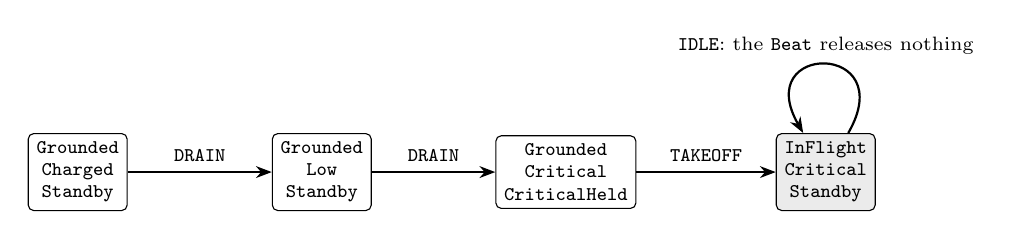
\begin{tikzpicture}[
    st/.style={draw, rounded corners=2pt, align=center, inner sep=3pt, font=\scriptsize},
    ar/.style={-{Stealth[length=2mm]}, thick},
    lb/.style={font=\scriptsize}
]
\node[st] (s0) at (0,0) {\code{Grounded}\\\code{Charged}\\\code{Standby}};
\node[st] (s1) at (3.1,0) {\code{Grounded}\\\code{Low}\\\code{Standby}};
\node[st] (s2) at (6.2,0) {\code{Grounded}\\\code{Critical}\\\code{CriticalHeld}};
\node[st, fill=black!8] (s3) at (9.5,0) {\code{InFlight}\\\code{Critical}\\\code{Standby}};
\draw[ar] (s0) -- node[lb, above] {\code{DRAIN}} (s1);
\draw[ar] (s1) -- node[lb, above] {\code{DRAIN}} (s2);
\draw[ar] (s2) -- node[lb, above] {\code{TAKEOFF}} (s3);
\draw[ar] (s3) to[out=60,in=120,looseness=6] node[lb, above] {\code{IDLE}: the \code{Beat} releases nothing} (s3);
\end{tikzpicture}
\caption{The shortest path to a blind state under \code{OneSlot}, written as (avionics, battery, environment). Idle ticks leave the state unchanged forever.}
\label{fig:lasso}
\end{figure}

Table~\ref{tab:policies} compares the three policies. The property is checked over the whole graph: a state is \emph{forever blind} if some infinite path with arbitrary inputs stays airborne with a critical battery (the greatest fixed point of ``blind and having a blind successor'').

\begin{table}[t]
\caption{Environment policies over the closed-loop graph (20 inputs per tick).}
\label{tab:policies}
\small
\begin{tabular}{@{}lp{1.9cm}p{2.4cm}p{2.9cm}@{}}
\toprule
Policy & reachable states & blind under idle ticks & forever blind (any inputs) \\
\midrule
\code{OneSlot} (implemented in \crem{}) & 26 & 2 & 2 \\
\code{Queue} (oracle only) & 28 & 1 & 1 \\
\code{Level} (oracle only) & 26 & 0 & 0 \\
\bottomrule
\end{tabular}
\end{table}

A loss-free queue does not remove the defect; reacting to the level does, for every sequence and not only up to a bound. This turns an earlier bounded measurement (172 scenarios of up to 8 ticks over a reduced alphabet end in this situation under \code{OneSlot}, 0 under \code{Level}) into a statement about the whole graph. The smallest scenario on which the \crem{} loop diverges step by step from \code{Level} has four ticks: \code{DRAIN}, \code{DRAIN}, \code{TAKEOFF}, \code{IDLE}. With the recorded seed, the Hedgehog shrinker, started from scenarios of up to 40 ticks, also reached these four ticks; but shrinking only guarantees a local minimum, so it is the breadth-first search, not the shrinker, that establishes that no shorter scenario exists.

\subsection{A correction to a bounded conclusion}

The earlier bounded runs reported that dropping events when the slot is busy never changed the final state (0 of 87\,381 scenarios differing between \code{OneSlot} and \code{Queue}). That alphabet had no \code{LandedSignal} command and no tick combining a command with a battery event. Over the full alphabet, the product of the two policies has 282 reachable pairs, and in \textbf{232} of them the (avionics, battery) pair differs at the end of a tick. The smallest case has four ticks: \code{DRAIN}; \code{TAKEOFF DRAIN}; \code{LANDED}; \code{RECHARGE}. It ends with the avionics \code{Grounded} under \code{OneSlot}, which dropped the landing news while its slot held the touchdown, and \code{Shutdown} under \code{Queue}, which kept it. The earlier statement was true of the alphabet it was measured on; it was not a property of the model. This is the kind of conclusion that bounded enumeration over a reduced alphabet cannot support, and that closing the graph can.

\subsection{Property-based tests and mutants}

Hedgehog found the \crem{} trace equal to the oracle's in 5\,000 random closed-loop scenarios of up to 40 ticks and 3\,000 open-loop ones, and the trace properties of the original suite held in 3\,000 scenarios of up to 60 ticks. To check that the test can fail, four defects were injected into the oracle's table, which is equivalent to a defect in the implementation because the comparison is symmetric, and the oracle was also run with the \code{Level} policy against \crem{}. All five were detected and shrunk: a wrong destination (1 tick), an illegal edge (2), swapped events (1), a wrong output (3) and the \code{Level} policy against \crem{} (4).

\subsection{Model checking}

TLC closed the TLA+ model with 1\,143 distinct states (1\,638 generated). With \code{OneSlot}, it reports a violation of \code{NoPermanentBlindness} with a lasso counterexample that is the path of Fig.~\ref{fig:lasso}; without that property every other property holds. With \code{Level}, all properties hold. The set of triples with an empty queue has 26 elements and is \emph{identical} to the set reached by the Haskell exploration. Two independent routes, the \crem{} machines run at every triple and a TLA+ specification written from the tables, therefore reach the same state space and the same verdict on the battery policy. This lowers the risk of an error in one of the two; it does not lower the risk of an interpretation error common to both, since the same person wrote them. TLC checks the model, not the Haskell code.

\subsection{What each kind of evidence establishes}

Table~\ref{tab:evidence} summarises what each kind of evidence in this section does and does not establish; the right-hand column is as important as the left.

\begin{table}[t]
\caption{What each kind of evidence establishes in this case study.}
\label{tab:evidence}
\small
\begin{tabular}{@{}p{3.1cm}p{4.5cm}p{4.2cm}@{}}
\toprule
Evidence & Establishes & Does not establish \\
\midrule
Compiler (topology, exhaustiveness as error) & edges outside the topology and omitted pairs are rejected & right destination for an event; any sequence property \\
Table and oracle, exhaustive on pairs & implementation conforms to the table on all 16 and 9 pairs & that the table reflects real requirements \\
Closure of the closed-loop graph & equivalence and safety for any length, under the abstraction hypothesis; the blind state & correctness of \crem{}; real avionics \\
Property-based tests & divergences in random scenarios, with seeds and shrinking & absence of divergence outside the sample \\
TLC & the same verdicts on an independently written model & anything about the Haskell code itself \\
\bottomrule
\end{tabular}
\end{table}

\section{Discussion}
\label{sec:discussion}

\subsection{Lessons for \crem{} users}

\paragraph{Treat the type as a per-edge guarantee.} In our mutation experiment the compiler caught two of nine defects. Writing every equation without a wildcard and compiling exhaustiveness as an error is what makes one of the two work; H9 shows that a catch-all clause undoes it. The wrong destination on an allowed edge is the most dangerous because it is silent; the cheap defence is a table in which events appear, checked exhaustively against the actions.

\paragraph{Keep the provenance of each rule.} Of the 16 rows of the avionics table only four come from the requirements. The distinction between \texttt{REQ}, \texttt{CONV} and \texttt{MODEL} turned a vague worry (``is the specification right?'') into a short list of questions for a reviewer.

\paragraph{Close the graph instead of enumerating strings.} The state space between ticks was tiny. Exploring it to closure with the real machines took seconds, replaced a bounded claim by an unbounded one, and corrected a conclusion that a bounded run over a reduced alphabet had supported. We do not know how well this scales: it relies on a small, finite, observable state, and \code{withSomeSing} on every vertex requires a closed set of vertices.

\paragraph{Make the environment a first-class, reviewable object.} The defect we found is in the environment. A typed state-machine library makes the machines safe; it does not make the \emph{integration policy} between them safe. Writing that policy as a table of cues, holdings and releases, with the alternatives side by side, is what exposed it.

\paragraph{Did the functional style help?} In three specific ways: pure machines made the oracle and the exploration trivial to run on any state; algebraic types made the vocabulary closed, so the typed boundary has no unreachable case; and \code{Feedback} as an ordinary value let us run one tick from an arbitrary state. The price was that observing a vertex inside \code{Basic}, whose state type is existential, required wrapping the action (the observation is rebuilt with the same \code{AllowedTransition} proof, so no rule is rewritten).

\subsection{Closing the gap: other techniques}

Tying events to edges in the types is possible in principle with indexed monads \cite{atkey2009parameterised} or dependently typed languages \cite{brady2013idris}, and typestate \cite{strom1986typestate} is the classic formulation of protocol-dependent types. We did not evaluate these alternatives; our claim is narrower: with the library as it is, a table and an oracle give a reviewable account of the event--destination relation, and the closed-loop properties need an exploration or a model checker whichever type system is used.

\subsection{Threats to validity}
\label{sec:threats}

\paragraph{Authorship.} One person wrote the implementation, the table, the oracle and the TLA+ model. A misreading of the requirements could be in all of them. The table separates what the text says from what was assumed, but the review by the project's supervisor is pending and there is no third-party oracle.

\paragraph{The abstraction hypothesis.} The ``any length'' claims depend on the loop's future being a function of the vertex triple. It holds by construction and was checked on 8\,421 scenarios, but it is not proved.

\paragraph{Generalisation.} There is one topology of four vertices and an environment with one slot. We did not vary topologies or scales, and the findings are about this model: the blind state is a property of the environment we wrote, not a defect of \crem{} or of GHC. The domain has no real requirements behind it.

\paragraph{Mutants and tools.} The mutants were chosen by the author. We used one version of each tool, one machine and one operating system. The shrinker finds local minima only.

\paragraph{Procedure.} The code, scripts and a first draft of this text were produced with the assistance of a generative AI system (see the statement below); every number comes from a recorded run, and the test suites include injected defects and hand-corrupted traces so that the checks demonstrably can fail.

\section{Related work}
\label{sec:related}

This section is a pointed discussion, not a systematic review; a systematic search was planned (its protocol is in the artefact) but has not been performed, and no claim of novelty is made beyond the delimitation stated in the introduction.

Typed finite-state machines in Haskell have been explored through indexed monads \cite{atkey2009parameterised}, the \texttt{motor} library \cite{motor} and \crem{} \cite{perone2023crem}; the latter lifts a topology to the type level with singletons \cite{eisenberg2012singletons}, and its authors note that the topology is not tied to the inputs. Typestate \cite{strom1986typestate} is the long-standing idea of types that change with protocol state. Property-based testing \cite{claessen2000quickcheck,hedgehog} and model checking with TLA+ \cite{lamport2002specifying,tlaplus} are the standard complements for behaviour that types do not cover; what we add is a concrete instance on a composed, fed-back typed machine, including a way to run the real machines from any state. The case of finite-state machines in pure functional languages was also treated by Malakhovski and Shalyto \cite{malakhovski2009fsm}; we cite it for the general idea only.

\section{Conclusion}

A type-level topology is a precise and useful guarantee, and it is a guarantee about edges. In a composed, fed-back system with an environment, the properties that matter are about sequences, and they can fail with every edge correct. In our case study the compiler rejected two of nine injected defects, a table-driven oracle and property-based tests caught the rest, and an exhaustive exploration of the real closed loop found a defect no edge-level check can see, which an independent TLA+ model reproduced. The reusable part is the method: a table with provenance, an oracle driven by it, a typed boundary, property-based tests, and closing the state graph by running the real machines from any vertex triple. What remains open is the independence of the specification from its author, other topologies and scales, and a systematic comparison with other approaches to the event--destination gap.

\section*{Data availability statement}

The code, tables, scenarios, TLA+ specification, scripts and all logs are in the artefact of this work: a frozen snapshot of the \texttt{avionics-crem} repository (commit \texttt{9689ce8}) plus the package \texttt{avionics-validation}. \textbf{[Public repository URL and archived DOI to be added before submission; the repository was private at the time of writing.]} A single script (\texttt{run\_all.sh}) rebuilds and reruns everything; \texttt{cabal.project.freeze} fixes the dependency versions.

\section*{Declaration of generative AI use}

Generative AI (Claude, Anthropic, through Claude Code) was used at the author's request to write the Haskell validation package, the scripts, the TLA+ specification and a first draft of this text, and to run the commands whose results are reported. \textbf{[The author to state the extent of his own review of code, results and text, and confirm compliance with the policy of the journal and of his institution.]} The results are from recorded runs; the author remains responsible for the content.

\section*{Funding and competing interests}

\textbf{[To be completed by the author.]}

\bibliographystyle{ACM-Reference-Format}
\bibliography{refs}

\end{document}
